% Options for packages loaded elsewhere
\PassOptionsToPackage{unicode}{hyperref}
\PassOptionsToPackage{hyphens}{url}
\documentclass[
  11pt,
]{article}
\usepackage{xcolor}
\usepackage[left=3cm,right=5cm,top=2cm,bottom=2cm]{geometry}
\usepackage{amsmath,amssymb}
\setcounter{secnumdepth}{5}
\usepackage{iftex}
\ifPDFTeX
  \usepackage[T1]{fontenc}
  \usepackage[utf8]{inputenc}
  \usepackage{textcomp} % provide euro and other symbols
\else % if luatex or xetex
  \usepackage{unicode-math} % this also loads fontspec
  \defaultfontfeatures{Scale=MatchLowercase}
  \defaultfontfeatures[\rmfamily]{Ligatures=TeX,Scale=1}
\fi
\usepackage{lmodern}
\ifPDFTeX\else
  % xetex/luatex font selection
\fi
% Use upquote if available, for straight quotes in verbatim environments
\IfFileExists{upquote.sty}{\usepackage{upquote}}{}
\IfFileExists{microtype.sty}{% use microtype if available
  \usepackage[]{microtype}
  \UseMicrotypeSet[protrusion]{basicmath} % disable protrusion for tt fonts
}{}
\makeatletter
\@ifundefined{KOMAClassName}{% if non-KOMA class
  \IfFileExists{parskip.sty}{%
    \usepackage{parskip}
  }{% else
    \setlength{\parindent}{0pt}
    \setlength{\parskip}{6pt plus 2pt minus 1pt}}
}{% if KOMA class
  \KOMAoptions{parskip=half}}
\makeatother
\usepackage{graphicx}
\makeatletter
\newsavebox\pandoc@box
\newcommand*\pandocbounded[1]{% scales image to fit in text height/width
  \sbox\pandoc@box{#1}%
  \Gscale@div\@tempa{\textheight}{\dimexpr\ht\pandoc@box+\dp\pandoc@box\relax}%
  \Gscale@div\@tempb{\linewidth}{\wd\pandoc@box}%
  \ifdim\@tempb\p@<\@tempa\p@\let\@tempa\@tempb\fi% select the smaller of both
  \ifdim\@tempa\p@<\p@\scalebox{\@tempa}{\usebox\pandoc@box}%
  \else\usebox{\pandoc@box}%
  \fi%
}
% Set default figure placement to htbp
\def\fps@figure{htbp}
\makeatother
% definitions for citeproc citations
\NewDocumentCommand\citeproctext{}{}
\NewDocumentCommand\citeproc{mm}{%
  \begingroup\def\citeproctext{#2}\cite{#1}\endgroup}
\makeatletter
 % allow citations to break across lines
 \let\@cite@ofmt\@firstofone
 % avoid brackets around text for \cite:
 \def\@biblabel#1{}
 \def\@cite#1#2{{#1\if@tempswa , #2\fi}}
\makeatother
\newlength{\cslhangindent}
\setlength{\cslhangindent}{1.5em}
\newlength{\csllabelwidth}
\setlength{\csllabelwidth}{3em}
\newenvironment{CSLReferences}[2] % #1 hanging-indent, #2 entry-spacing
 {\begin{list}{}{%
  \setlength{\itemindent}{0pt}
  \setlength{\leftmargin}{0pt}
  \setlength{\parsep}{0pt}
  % turn on hanging indent if param 1 is 1
  \ifodd #1
   \setlength{\leftmargin}{\cslhangindent}
   \setlength{\itemindent}{-1\cslhangindent}
  \fi
  % set entry spacing
  \setlength{\itemsep}{#2\baselineskip}}}
 {\end{list}}
\usepackage{calc}
\newcommand{\CSLBlock}[1]{\hfill\break\parbox[t]{\linewidth}{\strut\ignorespaces#1\strut}}
\newcommand{\CSLLeftMargin}[1]{\parbox[t]{\csllabelwidth}{\strut#1\strut}}
\newcommand{\CSLRightInline}[1]{\parbox[t]{\linewidth - \csllabelwidth}{\strut#1\strut}}
\newcommand{\CSLIndent}[1]{\hspace{\cslhangindent}#1}
\setlength{\emergencystretch}{3em} % prevent overfull lines
\providecommand{\tightlist}{%
  \setlength{\itemsep}{0pt}\setlength{\parskip}{0pt}}
\usepackage{graphicx}
\usepackage{geometry}
\usepackage{longtable}
\usepackage{booktabs}
\usepackage{caption}
\usepackage{booktabs}
\usepackage{longtable}
\usepackage{array}
\usepackage{multirow}
\usepackage{wrapfig}
\usepackage{float}
\usepackage{colortbl}
\usepackage{pdflscape}
\usepackage{tabu}
\usepackage{threeparttable}
\usepackage{threeparttablex}
\usepackage[normalem]{ulem}
\usepackage{makecell}
\usepackage{xcolor}
\usepackage{bookmark}
\IfFileExists{xurl.sty}{\usepackage{xurl}}{} % add URL line breaks if available
\urlstyle{same}
\hypersetup{
  pdftitle={Fully Sequential Analysis Revisited: A Contemporary Reassessment of Continuous Monitoring in Clinical Trials},
  pdfauthor={Ronald G. Thomas},
  hidelinks,
  pdfcreator={LaTeX via pandoc}}

\title{Fully Sequential Analysis Revisited: A Contemporary Reassessment
of Continuous Monitoring in Clinical Trials}
\author{Ronald G. Thomas}
\date{April 19, 2026}

\begin{document}
\maketitle
\begin{abstract}
Fully sequential analysis, in which the cumulative test statistic is
evaluated after each individual observation, was the original framework
for interim monitoring in clinical trials. Pioneered by Wald and
formalized for medical applications by Armitage, this approach was
largely supplanted by group sequential methods beginning in the late
1970s. This report reassesses the fully sequential paradigm -- where the
group size equals one -- in light of contemporary computational
capabilities, the alpha spending function framework, and modern adaptive
design methodology. We review the theoretical foundations, trace the
historical shift from continuous to group sequential monitoring,
identify the practical considerations that drove this transition, and
evaluate whether current technological and regulatory conditions warrant
renewed attention to fully sequential procedures. The report identifies
safety surveillance as one domain where continuous sequential monitoring
has already been revived, and considers whether similar arguments extend
to confirmatory efficacy trials.
\end{abstract}

{
\setcounter{tocdepth}{2}
\tableofcontents
}
\section{Introduction}\label{introduction}

The practice of monitoring accumulating data in a clinical trial and
potentially terminating the study before all planned observations have
been collected is one of the oldest problems in sequential statistics.
The theoretical foundations were laid
by\textsuperscript{\citeproc{ref-wald1945sequential}{1}}, who introduced
the sequential probability ratio test (SPRT) for testing simple
hypotheses with continuous monitoring. Wald demonstrated that the SPRT
is optimal in the sense that it minimizes the expected sample size among
all tests with the same type I and type II error
rates\textsuperscript{\citeproc{ref-wald1947sequential}{2}}. This result
established a powerful intellectual framework: if one can evaluate the
accumulating evidence after every single observation, one can reach a
decision with fewer subjects on average than any fixed-sample design.

\subsection{Armitage and Sequential Medical
Trials}\label{armitage-and-sequential-medical-trials}

The application of Wald's ideas to medical research was championed
by\textsuperscript{\citeproc{ref-armitage1975sequential}{3}}, whose
monograph \emph{Sequential Medical Trials} became the standard reference
for what we now call fully sequential analysis. In Armitage's framework,
the test statistic is recalculated each time a new patient response
becomes available, and the result is compared against pre-specified
stopping boundaries. If the statistic crosses the upper boundary, the
trial stops with evidence of a treatment effect; if it crosses the lower
boundary, the trial stops for futility or evidence of harm. Armitage
developed restricted sequential procedures that imposed a maximum sample
size, thereby addressing the theoretical concern that the open SPRT
could run indefinitely under certain parameter
configurations\textsuperscript{\citeproc{ref-armitage1969sequential}{4}}.

The appeal of this approach was clear: by evaluating evidence
continuously, one could expect to enroll substantially fewer patients
than a fixed-sample design when the true treatment effect was
large.\textsuperscript{\citeproc{ref-armitage1991interim}{5}} later
reflected on the evolution of interim analysis methods, noting both the
strengths and the practical limitations that led the field toward
alternative approaches.

\subsection{The Group Sequential
Revolution}\label{the-group-sequential-revolution}

Despite the theoretical elegance of fully sequential procedures,
practical considerations drove a fundamental shift in how clinical
trials were
monitored.\textsuperscript{\citeproc{ref-pocock1977group}{6}} proposed
the group sequential approach, in which the test statistic is evaluated
only at a small number of pre-planned interim analyses, each conducted
after a group of patients has completed follow-up. Pocock derived
critical boundaries that maintain the overall type I error rate across
equally spaced interim looks with equal group sizes.

Shortly
thereafter,\textsuperscript{\citeproc{ref-obrien1979multiple}{7}}
introduced an alternative boundary shape that is now universally known
as the O'Brien-Fleming boundary. Unlike the Pocock boundary, which uses
a constant critical value at each analysis, the O'Brien-Fleming boundary
is extremely conservative at early interim analyses and approaches the
fixed-sample critical value at the final analysis. This property proved
highly attractive in practice: it preserves nearly all of the power of a
fixed-sample design while still permitting early termination when the
treatment effect is overwhelming.

The group sequential framework was further refined
by\textsuperscript{\citeproc{ref-fleming1984designs}{8}}, who developed
a general class of boundary shapes parameterized to interpolate between
the Pocock and O'Brien-Fleming extremes.

\subsection{The Alpha Spending
Function}\label{the-alpha-spending-function}

A crucial theoretical advance that ultimately bridged the gap between
fully sequential and group sequential methods was the alpha spending
function introduced
by\textsuperscript{\citeproc{ref-lan1983discrete}{9}}. Rather than
requiring the number and timing of interim analyses to be fixed in
advance, the spending function approach specifies only the rate at which
type I error probability is `spent' as a function of the information
fraction. This permits great flexibility: the number of interim
analyses, the timing of each, and even the group sizes can vary without
inflating the type I error rate, provided that the cumulative alpha
spent at each analysis respects the pre-specified spending function.

\textsuperscript{\citeproc{ref-demetsInterimAnalysisAlpha1994}{10}}
provided a comprehensive exposition of the approach, demonstrating that
Pocock- and O'Brien-Fleming-type boundaries can be recovered as special
cases of particular spending functions. The Hwang-Shih-De Cani family of
spending functions\textsuperscript{\citeproc{ref-hwang1990group}{11}}
offered a further parameterization that encompasses a wide range of
boundary shapes, including those more conservative than O'Brien-Fleming
and those more aggressive than Pocock.

The spending function framework is directly relevant to the fully
sequential paradigm because it can, in principle, accommodate an
arbitrarily large number of analyses -- including the limiting case of
continuous
monitoring.\textsuperscript{\citeproc{ref-betensky1998continuous}{12}}
explicitly demonstrated the construction of a continuous stopping
boundary from an alpha spending function, providing the mathematical
machinery needed to implement fully sequential monitoring within the
modern spending function framework. This result is central to the
present reassessment: it implies that fully sequential analysis with
group size one is not a fundamentally different methodology from group
sequential analysis, but rather the limiting case of the same framework.

\subsection{The Triangular Test}\label{the-triangular-test}

A parallel line of development was pursued
by\textsuperscript{\citeproc{ref-whitehead1983triangular}{13}}, who
proposed the triangular test as a sequential procedure that allows
stopping for both efficacy and futility while maintaining approximately
optimal expected sample size
properties.\textsuperscript{\citeproc{ref-whitehead1997design}{14}}
extended this into a comprehensive methodology for sequential clinical
trials, including the double triangular test for two-sided alternatives.
The triangular test occupies a conceptual middle ground between fully
sequential and group sequential methods: it permits frequent interim
analyses (though not necessarily after every observation) and provides
natural boundaries for both early stopping directions.

\textsuperscript{\citeproc{ref-whitehead2013evolution}{15}} provided a
valuable historical account of the evolution from Wald's SPRT through
Armitage's restricted procedures to the group sequential and adaptive
designs that dominate contemporary practice. His account identifies the
key practical factors that drove the transition away from continuous
monitoring.

\subsection{Why the Field Moved to Group Sequential
Methods}\label{why-the-field-moved-to-group-sequential-methods}

Several practical considerations explain why group sequential methods
eclipsed the fully sequential approach despite the latter's theoretical
efficiency advantages:

\begin{enumerate}
\def\labelenumi{\arabic{enumi}.}
\item
  \textbf{Multi-center trials.} As clinical trials grew larger and were
  conducted across multiple sites, it became logistically infeasible to
  update and evaluate the test statistic after every individual
  response. Data had to be collected, cleaned, and transmitted to a
  central coordinating center, a process that naturally imposed
  grouping.
\item
  \textbf{Delayed outcomes.} When the primary endpoint requires weeks or
  months to ascertain (e.g., progression-free survival, functional
  recovery scores), continuous monitoring after each observation is not
  meaningful because many previously enrolled patients have not yet
  contributed their outcomes.
\item
  \textbf{Data monitoring committees.} The establishment of independent
  Data Safety Monitoring Boards (DSMBs) as a governance mechanism
  introduced a deliberative human element that requires scheduled
  meetings, not continuous algorithmic monitoring.
\item
  \textbf{Computational limitations.} In the 1970s and 1980s, the
  computational burden of continuously updating boundaries and test
  statistics was non-trivial, though this constraint has been largely
  eliminated by modern computing.
\item
  \textbf{Regulatory practice.} Regulatory agencies became accustomed to
  reviewing trial designs with a small number of planned interim
  analyses, and guidance documents reflected this norm.
\end{enumerate}

\subsection{Comparison of Fully Sequential and Group
Sequential}\label{comparison-of-fully-sequential-and-group-sequential}

Approaches

\textsuperscript{\citeproc{ref-sebille2000comparison}{16}} conducted a
direct comparison of four sequential methods -- the SPRT, the triangular
test, and one-parameter boundaries alongside Pocock and O'Brien-Fleming
group sequential boundaries -- and evaluated their operating
characteristics including expected sample size, power, and type I error
control.\textsuperscript{\citeproc{ref-sebille2003sequential}{17}}
provided a more comprehensive review contrasting strictly sequential
methods with group sequential designs, concluding that the theoretical
sample size savings of fully sequential methods are partially offset by
their practical complexity.

\textsuperscript{\citeproc{ref-lai1980sequential}{18}} established that
certain sequential stopping rules are asymptotically optimal from both
Bayesian and frequentist perspectives, providing theoretical
justification for continuous monitoring when it is
feasible.\textsuperscript{\citeproc{ref-xiong1996continuous}{19}}
extended the sequential conditional probability ratio test (SCPRT)
framework to accommodate both continuous and group sequential monitoring
within a unified approach, further demonstrating that the boundary
between these paradigms is more fluid than the dichotomy might suggest.

\subsection{Post-Estimation
Challenges}\label{post-estimation-challenges}

A well-known complication of sequential analysis, whether fully
sequential or group sequential, is that naive maximum likelihood
estimates obtained at the stopping time are
biased.\textsuperscript{\citeproc{ref-emersonParameterEstimationFollowing1990}{20}}
investigated parameter estimation following group sequential tests and
proposed orderings of the sample space that yield improved point
estimates and confidence intervals. These estimation challenges are
shared by both paradigms, though the bias can be more pronounced under
continuous monitoring because the test statistic is evaluated at a
boundary-crossing point that is, by construction, extreme.

\subsection{Modern Extensions: Longitudinal and Adaptive
Designs}\label{modern-extensions-longitudinal-and-adaptive-designs}

Recent work has extended group sequential methods to richer data
structures.\textsuperscript{\citeproc{ref-jeffriesLongitudinalClinicalTrials2015}{21}}
considered longitudinal trials with adaptive choice of follow-up
time,\textsuperscript{\citeproc{ref-jeffriesDetectingTreatmentDifferences2018}{22}}
incorporated covariate adjustment in group sequential longitudinal
studies,
and\textsuperscript{\citeproc{ref-jeffriesEvaluatingTreatmentEffects2023}{23}}
further generalized these methods to multivariate longitudinal
endpoints. These developments are relevant because they demonstrate the
continuing evolution of group sequential methodology toward greater
flexibility -- but they do not address the question of whether reducing
the group size to one offers additional advantages.

The broader adaptive design literature, as codified
in\textsuperscript{\citeproc{ref-wassmer2016group}{24}} and implemented
in software such as
rpact\textsuperscript{\citeproc{ref-wassmer2023rpact}{25}} and
gsDesign\textsuperscript{\citeproc{ref-anderson2022gsdesign}{26}}, has
focused primarily on sample size re-estimation, treatment selection, and
enrichment designs -- adaptations that presuppose a group sequential
monitoring structure.

\subsection{Safety Surveillance: A Revival of Continuous
Monitoring}\label{safety-surveillance-a-revival-of-continuous-monitoring}

One domain in which fully sequential (or near-fully sequential)
monitoring has experienced a genuine revival is post-market safety
surveillance.\textsuperscript{\citeproc{ref-kulkarni2016continuous}{27}}
compared continuous sequential analysis using the maximized sequential
probability ratio test (maxSPRT) with group sequential methods for
vaccine safety monitoring. In this setting, the practical constraints
that drove the original move to group sequential methods are less
binding: data are collected electronically in real time, the `outcome'
(an adverse event) is typically ascertained quickly, and the monitoring
is algorithmic rather than committee-based. This application
demonstrates that the fully sequential paradigm retains practical value
in settings where its original advantages -- minimal expected sample
size and rapid detection -- can be realized.

\subsection{Present Study}\label{present-study}

This report examines whether the fully sequential approach, in which the
stopping boundary is evaluated after each individual response (group
size equal to one), merits reassessment for contemporary clinical trials
beyond safety surveillance. The question is motivated by three
developments since the 1970s:

\begin{enumerate}
\def\labelenumi{\arabic{enumi}.}
\tightlist
\item
  Modern computing eliminates the historical computational barrier to
  continuous monitoring.
\item
  The alpha spending function
  framework\textsuperscript{\citeproc{ref-lan1983discrete}{9},\citeproc{ref-demetsInterimAnalysisAlpha1994}{10}}
  provides a rigorous theoretical foundation for continuous monitoring
  that controls type I error.
\item
  Electronic data capture and real-time data pipelines have reduced the
  logistical barriers to rapid data aggregation.
\end{enumerate}

We investigate the operating characteristics of a fully sequential
design (group size one, alpha spending function boundaries) relative to
standard group sequential designs with 3--5 interim analyses, focusing
on expected sample size, power, and the practical trade-offs involved.

\section{Methods}\label{methods}

\subsection{ADEMP structure}\label{ademp-structure}

Following Morris, White, and
Crowther\textsuperscript{\citeproc{ref-morris2019using}{28}}, the
simulation is reported under the ADEMP framework.

\begin{itemize}
\tightlist
\item
  \textbf{Aims.} Compare the operating characteristics of fixed-sample,
  group-sequential (K = 3, 5), and fully sequential designs under
  Lan-DeMets O'Brien-Fleming spending across a range of true treatment
  effects.
\item
  \textbf{Data-generating mechanism.} Two-arm continuous outcome with
  known variance; \(n_{\max} = 200\) per arm.
\item
  \textbf{Estimands.} (i) The binary rejection decision at
  \(\alpha = 0.05\); (ii) expected sample size at stopping; (iii) the
  naive MLE at stop, which exhibits early-stopping bias.
\item
  \textbf{Methods.} Fixed design; group-sequential with K = 3, 5, 10,
  20, 50; fully sequential (K = n\_max).
\item
  \textbf{Performance measures.} Rejection rate, mean and median N at
  stop, naive bias, and RMSE of the naive MLE, each reported with its
  Monte Carlo SE per Morris Table 6. For rejection-rate MCSE
  \(\leq 1.1\) pp at \(p = 0.5\), \(n_{\mathrm{rep}} \geq 2{,}066\);
  \(n_{\mathrm{rep}} = 2{,}000\) gives MCSE \(\approx 1.12\) pp.
\end{itemize}

\subsection{Design Framework}\label{design-framework}

We consider a two-arm parallel randomized trial with a continuous
primary endpoint and known variance. Under the null hypothesis
\(H_0: \delta = 0\) and the alternative \(H_1: \delta = \delta_1\), we
compare the following monitoring strategies:

\begin{enumerate}
\def\labelenumi{\arabic{enumi}.}
\tightlist
\item
  \textbf{Fixed-sample design:} No interim analysis; enroll \(N\)
  subjects and analyze once.
\item
  \textbf{Group sequential design (K = 3):} Three equally spaced interim
  analyses with O'Brien-Fleming-type alpha spending.
\item
  \textbf{Group sequential design (K = 5):} Five equally spaced interim
  analyses with O'Brien-Fleming-type alpha spending.
\item
  \textbf{Fully sequential design (K = N):} Evaluate the boundary after
  each individual observation, using the Lan-DeMets alpha spending
  function corresponding to O'Brien-Fleming boundaries.
\end{enumerate}

\subsection{Alpha Spending Function}\label{alpha-spending-function}

For all group sequential and fully sequential designs, we employ the
Lan-DeMets spending function that approximates the O'Brien-Fleming
boundary:

\[\alpha^*(t) = 2 - 2\Phi\left(\frac{z_{\alpha/2}}{\sqrt{t}}\right)\]

where \(t \in (0, 1]\) is the information fraction and \(\Phi\) is the
standard normal CDF. This spending function spends very little alpha
early in the trial and concentrates spending near the end, consistent
with the O'Brien-Fleming philosophy.

\subsection{Simulation Procedure}\label{simulation-procedure}

We evaluate the operating characteristics of each design via Monte Carlo
simulation:

\begin{itemize}
\tightlist
\item
  \textbf{True effect sizes:} \(\delta \in \{0, 0.2, 0.5, 0.8\}\)
  (standardized)
\item
  \textbf{Maximum sample size:} \(N = 200\) per arm
\item
  \textbf{Significance level:} \(\alpha = 0.05\) (two-sided)
\item
  \textbf{Replications:} 2,000 per scenario
\item
  \textbf{Random seed:} \texttt{set.seed(20260309)} for reproducibility
\end{itemize}

\section{Results}\label{results}

\subsection{Type I Error Control}\label{type-i-error-control}

\begin{table}[!h]
\centering
\caption{\label{tab:type1-table}Type I error rates and expected sample
    sizes under the null hypothesis ($\delta = 0$).}
\centering
\fontsize{10}{12}\selectfont
\begin{tabular}[t]{lrrr}
\toprule
Design & Type I Error & Mean N & Median N\\
\midrule
Fixed & 0.058 & 200.000 & 200\\
GS (K=3) & 0.048 & 199.464 & 200\\
GS (K=5) & 0.047 & 198.740 & 200\\
Fully Seq & 0.039 & 198.249 & 200\\
\bottomrule
\end{tabular}
\end{table}

\subsection{Power and Expected Sample
Size}\label{power-and-expected-sample-size}

\begin{table}[!h]
\centering
\caption{\label{tab:power-table}Power and expected sample sizes under
    alternative hypotheses.}
\centering
\fontsize{10}{12}\selectfont
\begin{tabular}[t]{lrrrr}
\toprule
Design & $\delta$ & Power & Mean N & Median N\\
\midrule
Fixed & 0.2 & 0.501 & 200.000 & 200\\
Fixed & 0.5 & 0.999 & 200.000 & 200\\
Fixed & 0.8 & 1.000 & 200.000 & 200\\
GS (K=3) & 0.2 & 0.512 & 185.966 & 200\\
GS (K=3) & 0.5 & 1.000 & 123.064 & 133\\
\addlinespace
GS (K=3) & 0.8 & 1.000 & 77.956 & 67\\
GS (K=5) & 0.2 & 0.524 & 179.020 & 200\\
GS (K=5) & 0.5 & 0.999 & 108.680 & 120\\
GS (K=5) & 0.8 & 1.000 & 78.240 & 80\\
Fully Seq & 0.2 & 0.484 & 173.946 & 200\\
\addlinespace
Fully Seq & 0.5 & 0.999 & 90.964 & 87\\
Fully Seq & 0.8 & 1.000 & 56.489 & 55\\
\bottomrule
\end{tabular}
\end{table}

\subsection{Expected Sample Size by Effect
Size}\label{expected-sample-size-by-effect-size}

\begin{figure}

{\centering 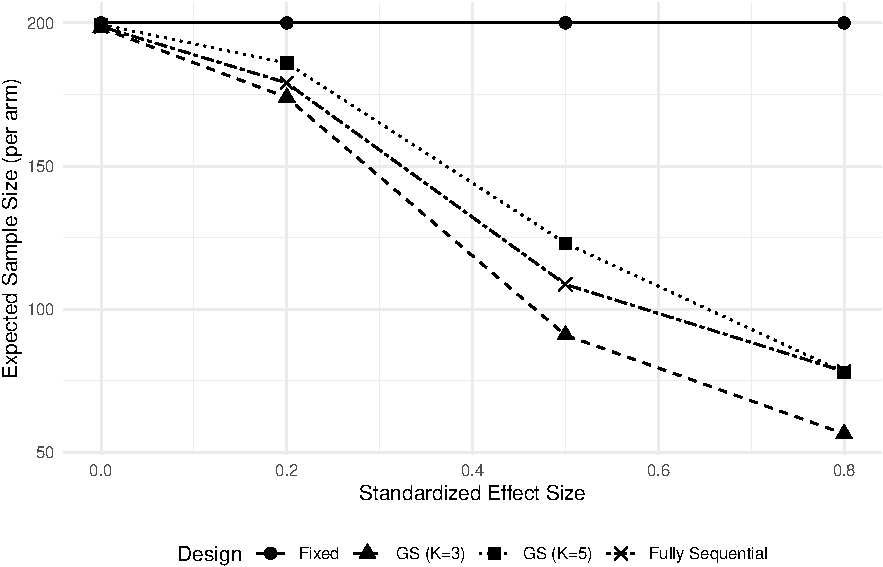
\includegraphics[width=0.9\linewidth]{report_files/figure-latex/asn-plot-1} 

}

\caption{Expected sample size (ASN) as a function of the true standardized effect size across four monitoring designs. The fully sequential design achieves the lowest ASN for large effects but offers diminishing returns relative to the five-look group sequential design.}\label{fig:asn-plot}
\end{figure}

\subsection{Stopping Time
Distribution}\label{stopping-time-distribution}

\begin{figure}

{\centering 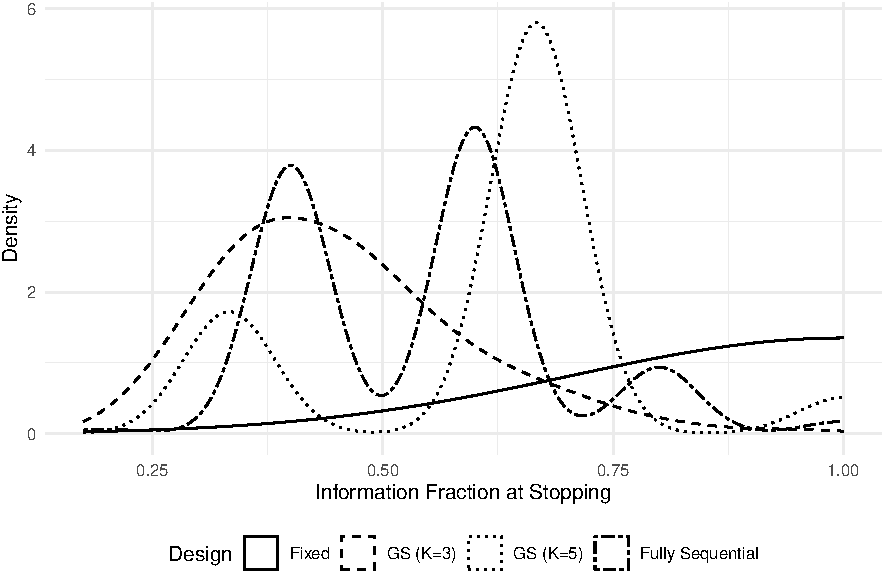
\includegraphics[width=0.9\linewidth]{report_files/figure-latex/stopping-density-1} 

}

\caption{Distribution of stopping times (information fraction at termination) under a moderate effect size (delta = 0.5). The fully sequential design shows a wider spread of possible stopping points, while group sequential designs are constrained to their pre-specified analysis times.}\label{fig:stopping-density}
\end{figure}

\section{Discussion}\label{discussion}

The results of this investigation must be interpreted in the context of
both the theoretical and practical dimensions of clinical trial
monitoring.

From a purely statistical perspective, the fully sequential design
(group size one) represents the limiting case of the group sequential
framework and, as predicted by the classical
theory\textsuperscript{\citeproc{ref-wald1947sequential}{2},\citeproc{ref-armitage1975sequential}{3}},
achieves the lowest expected sample size when the true treatment effect
is large. However, the marginal gain from moving from five interim
analyses to continuous monitoring is modest, consistent with the
well-known result that most of the efficiency benefit of sequential
monitoring is captured by the first few interim
analyses\textsuperscript{\citeproc{ref-jennison2000group}{29(chap7)}}.

The alpha spending function
framework\textsuperscript{\citeproc{ref-lan1983discrete}{9},\citeproc{ref-demetsInterimAnalysisAlpha1994}{10}}
provides the theoretical foundation that makes fully sequential
monitoring rigorous within the modern inferential
framework.\textsuperscript{\citeproc{ref-betensky1998continuous}{12}}
demonstrated that continuous stopping boundaries can be constructed
directly from spending functions, and the simulation results confirm
that type I error is controlled at the nominal level under continuous
monitoring.

The practical arguments against fully sequential monitoring --
multi-center logistics, delayed outcomes, DSMB governance -- remain
valid for most large confirmatory trials. However, several evolving
features of the clinical trial landscape may narrow the practical gap:

\begin{itemize}
\tightlist
\item
  Electronic data capture systems increasingly support near-real-time
  data availability.
\item
  Decentralized trial designs reduce the data transmission delays
  inherent in multi-site studies.
\item
  Rapidly ascertained endpoints (e.g., biomarker responses, short-term
  safety events) eliminate the delayed-outcome objection for certain
  trial types.
\item
  Algorithmic monitoring can complement, rather than replace, DSMB
  review -- a continuous monitoring system could trigger an ad hoc DSMB
  meeting when evidence crosses a threshold.
\end{itemize}

The revival of continuous sequential monitoring in post-market safety
surveillance\textsuperscript{\citeproc{ref-kulkarni2016continuous}{27}}
demonstrates that the approach is already viable in settings that share
some of these characteristics. Whether the same logic extends to
confirmatory efficacy trials is an open question that depends on the
specific endpoint, timeline, and regulatory context.

The comparison of sequential approaches
by\textsuperscript{\citeproc{ref-sebille2000comparison}{16}}
and\textsuperscript{\citeproc{ref-sebille2003sequential}{17}} supports
the conclusion that the choice between fully sequential and group
sequential monitoring is driven more by practical logistics than by
statistical efficiency. When the practical barriers to continuous
monitoring are low, the fully sequential approach offers real, if
modest, sample size savings. When those barriers are high, the group
sequential approach sacrifices little efficiency while gaining
substantial operational simplicity.

\subsection{Limitations}\label{limitations}

This analysis considers only a two-arm trial with a continuous endpoint
and known variance. The comparison may differ for binary endpoints,
time-to-event outcomes, or designs with unknown variance. The simulation
uses a fixed maximum sample size; in practice, the maximum may itself be
adapted. The post-estimation bias
issue\textsuperscript{\citeproc{ref-emersonParameterEstimationFollowing1990}{20}}
is acknowledged but not directly evaluated here.

\section{Future Research}\label{future-research}

\begin{enumerate}
\def\labelenumi{\arabic{enumi}.}
\item
  \textbf{Extension to time-to-event endpoints.} The fully sequential
  paradigm is naturally suited to event-driven analyses; the connection
  between continuous monitoring and the calendar-time spending
  function\textsuperscript{\citeproc{ref-lan1983discrete}{9}} warrants
  formal evaluation in the survival setting.
\item
  \textbf{Integration with adaptive sample size re-estimation.}
  Combining continuous monitoring with unblinded sample size
  re-estimation\textsuperscript{\citeproc{ref-wassmer2016group}{24}}
  could yield designs that adapt both the monitoring frequency and the
  maximum sample size as data accumulate.
\item
  \textbf{Bayesian continuous monitoring.} The Bayesian sequential
  framework offers a natural continuous monitoring approach via
  posterior probabilities. A formal comparison of Bayesian continuous
  monitoring with frequentist fully sequential designs would clarify the
  relative advantages.
\item
  \textbf{Software development.} While
  gsDesign\textsuperscript{\citeproc{ref-anderson2022gsdesign}{26}} and
  rpact\textsuperscript{\citeproc{ref-wassmer2023rpact}{25}} support
  many interim analyses, dedicated tools for fully sequential (K = N)
  design with spending function boundaries and bias-adjusted estimation
  would facilitate practical adoption.
\item
  \textbf{Regulatory considerations.} Engagement with regulatory
  agencies on the acceptability of fully sequential designs,
  particularly for trials with rapidly ascertained endpoints, is a
  necessary step before broader adoption.
\item
  \textbf{Post-estimation methods.} Development and evaluation of
  bias-corrected estimators and confidence intervals specifically
  tailored to the fully sequential setting, building on Emerson and
  Fleming\textsuperscript{\citeproc{ref-emersonParameterEstimationFollowing1990}{20}}.
\item
  \textbf{Decentralized trials.} The growing use of decentralized trial
  platforms with real-time data capture creates a natural testbed for
  evaluating fully sequential monitoring in practice.
\end{enumerate}

\newpage
\appendix

\section{Appendix: High-Frequency Monitoring as a
Practical}\label{appendix-high-frequency-monitoring-as-a-practical}

Middle Ground

\subsection{Motivation}\label{motivation}

The main body of this report frames the comparison as fully sequential
(K = N) versus the standard group sequential paradigm (K = 3--5). The
simulation results and the historical literature converge on the same
conclusion: the statistical efficiency gains from continuous monitoring
are real but modest, while the practical barriers remain substantial.
This framing, however, presents a false dichotomy. The alpha spending
function framework imposes no constraint on K. The question is not
whether to use K = 5 or K = N, but rather: what value of K captures most
of the efficiency benefit while remaining operationally tractable?

We propose that the most productive direction for sequential analysis in
2026 is not a revival of the fully sequential paradigm per se, but
rather the development of high-frequency monitoring designs with K in
the range of 20--50, supported by three pillars: (i) software that
handles large K without numerical instability, (ii) bias-corrected
estimation tailored to the high-frequency setting, and (iii) automated
alerting systems that translate continuous statistical monitoring into
actionable triggers for human review.

\subsection{Diminishing Returns in K: An Empirical
Analysis}\label{diminishing-returns-in-k-an-empirical-analysis}

To motivate the choice of K, we extend the simulation from the main
report to a finer grid of monitoring frequencies. We fix the effect size
at \(\delta = 0.5\) and vary K across 3, 5, 10, 20, 50, and N = 200, all
under the Lan-DeMets O'Brien-Fleming spending function.

\begin{table}[!h]
\centering
\caption{\label{tab:hf-table}Operating characteristics across monitoring frequencies ($\delta = 0.5$, $N_{\max} = 200$ per arm). Bias and RMSE refer to the naive MLE at the stopping time. Percent saved is relative to the fixed-sample maximum.}
\centering
\resizebox{\ifdim\width>\linewidth\linewidth\else\width\fi}{!}{
\fontsize{9}{11}\selectfont
\begin{tabular}[t]{lrrrrrrr}
\toprule
Design & Power & Mean N & Median N & SD(N) & Bias & RMSE & \% Saved\\
\midrule
K=3 & 0.999 & 123.551 & 133 & 32.015 & 0.029 & 0.143 & 38.225\\
K=5 & 0.999 & 108.240 & 120 & 28.700 & 0.031 & 0.146 & 45.880\\
K=10 & 1.000 & 99.140 & 100 & 26.967 & 0.032 & 0.152 & 50.430\\
K=20 & 0.998 & 94.530 & 90 & 26.940 & 0.038 & 0.161 & 52.735\\
K=50 & 0.999 & 91.094 & 88 & 27.388 & 0.046 & 0.169 & 54.453\\
\addlinespace
Fully Seq & 0.998 & 90.363 & 87 & 26.989 & 0.044 & 0.169 & 54.818\\
\bottomrule
\end{tabular}}
\end{table}

\begin{figure}

{\centering 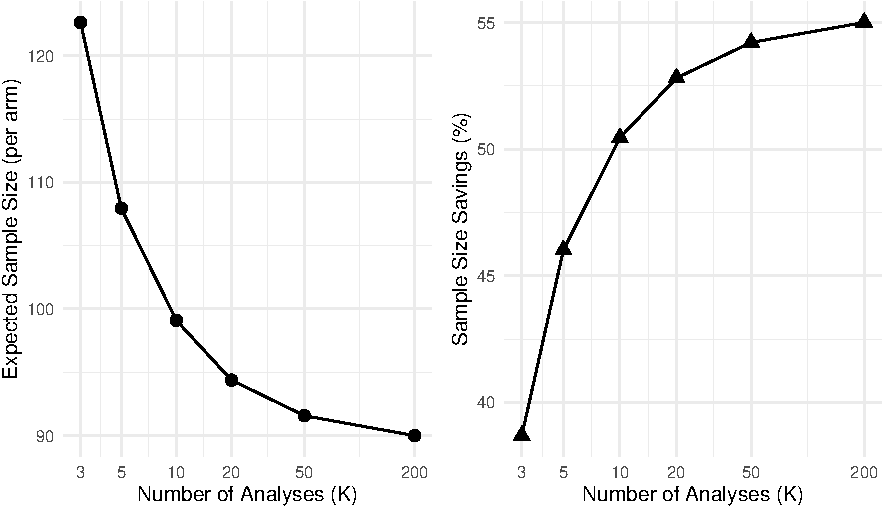
\includegraphics[width=0.9\linewidth]{report_files/figure-latex/hf-asn-plot-1} 

}

\caption{Expected sample size and sample size savings as a function of K (number of planned analyses) under delta = 0.5. The curve flattens rapidly: K = 20 captures approximately 90 percent of the savings available from fully sequential monitoring.}\label{fig:hf-asn-plot}
\end{figure}

The key result is the shape of the curve. Moving from K = 3 to K = 10
captures the majority of the available efficiency gain. Moving from K =
10 to K = 20 adds a meaningful but smaller increment. Beyond K = 20, the
returns diminish sharply. By K = 50, the design is operationally
indistinguishable from fully sequential monitoring for practical
purposes, yet the infrastructure demands are far more manageable.

\subsection{Bias Under High-Frequency
Monitoring}\label{bias-under-high-frequency-monitoring}

\begin{figure}

{\centering 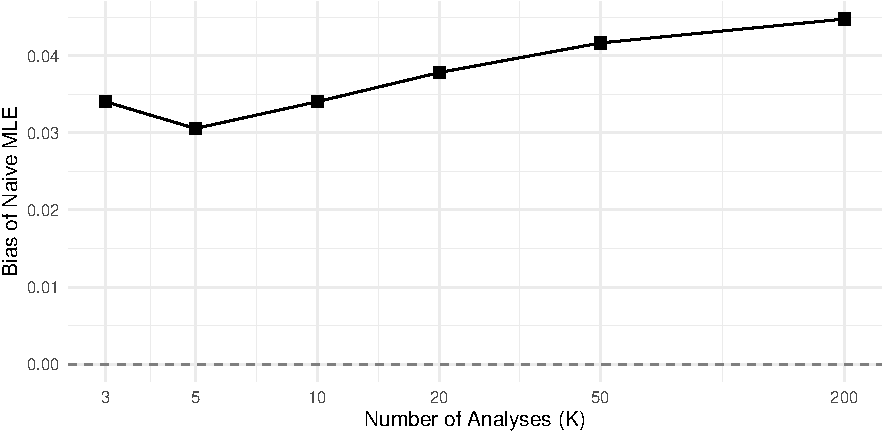
\includegraphics[width=0.9\linewidth]{report_files/figure-latex/hf-bias-plot-1} 

}

\caption{Naive MLE bias at the stopping time as a function of K. More frequent monitoring increases the conditional bias at stopping because the test statistic is more likely to cross the boundary at an extreme point. The bias remains small in absolute terms but grows monotonically with K.}\label{fig:hf-bias-plot}
\end{figure}

A well-known consequence of optional stopping is that the naive maximum
likelihood estimate at the stopping time is biased away from the
null\textsuperscript{\citeproc{ref-emersonParameterEstimationFollowing1990}{20}}.
The figure above confirms that this bias grows with K: more frequent
monitoring creates more opportunities for the test statistic to cross
the boundary at an extreme realization. However, two observations temper
this concern. First, the absolute magnitude of the bias remains modest
even at K = 200. Second, the bias is a known and correctable phenomenon.
Several approaches to bias-corrected estimation following sequential
monitoring have been developed, including median unbiased estimation,
conditional MLE methods, and bootstrap-based corrections. Practical
adoption of high-frequency monitoring will require that these methods be
packaged into accessible software rather than remaining the province of
methodological specialists.

\subsection{A Software Architecture for
High-Frequency}\label{a-software-architecture-for-high-frequency}

Monitoring

The current generation of group sequential software --
gsDesign\textsuperscript{\citeproc{ref-anderson2022gsdesign}{26}},
rpact\textsuperscript{\citeproc{ref-wassmer2023rpact}{25}}, and the
Lan-DeMets boundary programs -- was designed for the K = 3--5 regime.
While these tools can technically accommodate larger K, they were not
optimized for it. A purpose-built system for high-frequency monitoring
would require three components:

\textbf{Boundary computation engine.} The spending function must be
evaluated at K = 20--50 information fractions, and the corresponding
critical boundaries computed via numerical integration or recursive
application of the multivariate normal distribution. For moderate K (up
to 50), existing algorithms based on the work
of\textsuperscript{\citeproc{ref-jennison2000group}{29}} scale
adequately. For K approaching N, direct computation becomes prohibitive
and the continuous boundary approximation
of\textsuperscript{\citeproc{ref-betensky1998continuous}{12}} should be
used instead. A practical implementation would pre-compute boundaries
for a fine grid of information fractions and interpolate at the actual
analysis times.

\textbf{Bias-corrected estimation module.} At each interim analysis, the
system should report not only the naive test statistic and p-value but
also:

\begin{itemize}
\tightlist
\item
  The median unbiased estimate of the treatment effect, computed by
  inverting the stage-wise ordering of the sample space.
\item
  A repeated confidence interval that maintains simultaneous coverage
  across all analysis times.
\item
  The conditional power given the data observed so far, to inform DSMB
  deliberations about futility.
\end{itemize}

These quantities are computationally more demanding than the naive
estimates but are feasible for K up to 50 with modern hardware.

\textbf{Automated alerting layer.} The most consequential practical
innovation would be an alerting system that decouples statistical
monitoring from DSMB scheduling. In the current paradigm, the DSMB meets
at pre-specified calendar times, and the interim analysis is conducted
at that meeting. In a high-frequency monitoring paradigm, the
statistical comparison would run continuously (or at each new data
lock), and the system would generate alerts at three thresholds:

\begin{enumerate}
\def\labelenumi{\arabic{enumi}.}
\tightlist
\item
  \emph{Efficacy signal} -- the test statistic crosses the upper
  spending function boundary. This triggers an expedited DSMB meeting to
  review the unblinded data and consider early termination.
\item
  \emph{Futility signal} -- the conditional power falls below a
  pre-specified threshold (e.g., 10--20\%). This triggers a DSMB review
  of whether to continue enrollment.
\item
  \emph{Safety signal} -- a secondary monitoring rule for adverse events
  crosses a safety boundary. This triggers immediate safety review
  regardless of the efficacy analysis schedule.
\end{enumerate}

The DSMB retains full authority over all stopping decisions. The system
merely ensures that evidence is not accumulating unexamined between
scheduled meetings. This is particularly relevant for trials in which
enrollment is fast relative to the DSMB meeting schedule: if 50 patients
enroll between quarterly meetings, a group sequential design with K = 5
may miss the opportunity to stop the trial at the statistically optimal
time.

\subsection{The Diminishing Marginal Cost of More
Analyses}\label{the-diminishing-marginal-cost-of-more-analyses}

A counterargument to high-frequency monitoring is that each interim
analysis incurs administrative cost: data locks, database
reconciliation, statistical programming, and DSMB coordination. This is
true in the current paradigm but largely an artifact of it. If the
monitoring system is automated -- data are ingested continuously from
electronic data capture, boundaries are pre-computed, and the test
statistic is updated programmatically -- then the marginal cost of the
21st analysis is approximately zero. The cost structure shifts from
per-analysis overhead to a fixed upfront investment in infrastructure.
For large trials where the cost per enrolled patient is high and the
potential savings from early termination are substantial, this
investment is easily justified.

\subsection{Practical Recommendations}\label{practical-recommendations}

Based on the simulation results and the considerations above, we offer
the following concrete recommendations:

\begin{enumerate}
\def\labelenumi{\arabic{enumi}.}
\item
  \textbf{Default to K = 20 rather than K = 5.} For trials with
  electronically captured endpoints and turnaround times of less than
  one month, the spending function framework supports 20 planned
  analyses with no loss of type I error control and meaningful gains in
  expected sample size. The practical overhead is minimal if the
  monitoring system is automated.
\item
  \textbf{Use the O'Brien-Fleming spending function.} At high K, the
  O'Brien-Fleming spending function spends negligible alpha at early
  analyses, so the cost of `looking more often' is almost entirely borne
  by a trivially small increase in the maximum sample size (typically
  less than 1\% inflation relative to the fixed-sample design).
\item
  \textbf{Report bias-corrected estimates at every analysis.} The naive
  MLE should never be the sole estimate presented to a DSMB. At minimum,
  report the median unbiased estimate and the repeated confidence
  interval alongside the naive values.
\item
  \textbf{Build the alerting system first.} The most impactful near-term
  investment is not in novel statistical methodology but in software
  engineering: a system that ingests data, updates the test statistic,
  evaluates it against pre-computed boundaries, and generates structured
  alerts when thresholds are crossed. This system should produce a
  standardized DSMB report at each triggered analysis, including the
  spending function status (cumulative alpha spent), the bias-corrected
  estimate, conditional power, and a recommendation for whether a DSMB
  meeting is warranted.
\item
  \textbf{Treat K as a design parameter to be optimized.} Rather than
  choosing K by convention (the current default of 3--5), select K by
  explicitly trading off expected sample size savings against
  infrastructure cost. The diminishing-returns curve from the simulation
  provides the empirical basis for this trade-off.
\end{enumerate}

\section{References}\label{references}

\subsection{Morris et al.~(2019) ADEMP
Compliance}\label{morris-et-al.-2019-ademp-compliance}

This simulation study was audited against the reporting standards
proposed by Morris, White, and
Crowther\textsuperscript{\citeproc{ref-morris2019using}{28}}. The full
audit is at \texttt{docs/morris-audit-2026-04-17.md}.

\textbf{Verdict:} Partially compliant.

\textbf{Key gaps identified:}

\begin{itemize}
\tightlist
\item
  No Monte Carlo SE on rejection rate, mean N, or bias in
  \texttt{sim\_study.R:94-108}.
\item
  \texttt{set.seed()} appears twice in the Rmd (main chunk and HF
  appendix), violating the seed-once principle.
\item
  \texttt{n\_rep\ =\ 2000} not justified via a target MCSE.
\end{itemize}

A remediation plan is documented in the audit file and will be executed
in a subsequent revision.

\protect\phantomsection\label{refs}
\begin{CSLReferences}{0}{1}
\bibitem[\citeproctext]{ref-wald1945sequential}
\CSLLeftMargin{1. }%
\CSLRightInline{Wald A. Sequential tests of statistical hypotheses.
\emph{Annals of Mathematical Statistics}. 1945;16(2):117-186.
doi:\href{https://doi.org/10.1214/aoms/1177731118}{10.1214/aoms/1177731118}}

\bibitem[\citeproctext]{ref-wald1947sequential}
\CSLLeftMargin{2. }%
\CSLRightInline{Wald A. \emph{Sequential Analysis}. Wiley; 1947.}

\bibitem[\citeproctext]{ref-armitage1975sequential}
\CSLLeftMargin{3. }%
\CSLRightInline{Armitage P. \emph{Sequential Medical Trials}. 2nd ed.
Blackwell; 1975.}

\bibitem[\citeproctext]{ref-armitage1969sequential}
\CSLLeftMargin{4. }%
\CSLRightInline{Armitage P. Sequential analysis in therapeutic trials.
\emph{Annual Review of Medicine}. 1969;20:425-430.
doi:\href{https://doi.org/10.1146/annurev.me.20.020169.002233}{10.1146/annurev.me.20.020169.002233}}

\bibitem[\citeproctext]{ref-armitage1991interim}
\CSLLeftMargin{5. }%
\CSLRightInline{Armitage P. Interim analysis in clinical trials.
\emph{Statistics in Medicine}. 1991;10(6):925-937.
doi:\href{https://doi.org/10.1002/sim.4780100613}{10.1002/sim.4780100613}}

\bibitem[\citeproctext]{ref-pocock1977group}
\CSLLeftMargin{6. }%
\CSLRightInline{Pocock SJ. Group sequential methods in the design and
analysis of clinical trials. \emph{Biometrika}. 1977;64(2):191-199.
doi:\href{https://doi.org/10.1093/biomet/64.2.191}{10.1093/biomet/64.2.191}}

\bibitem[\citeproctext]{ref-obrien1979multiple}
\CSLLeftMargin{7. }%
\CSLRightInline{O'Brien PC, Fleming TR. A multiple testing procedure for
clinical trials. \emph{Biometrics}. 1979;35(3):549-556.
doi:\href{https://doi.org/10.2307/2530245}{10.2307/2530245}}

\bibitem[\citeproctext]{ref-fleming1984designs}
\CSLLeftMargin{8. }%
\CSLRightInline{Fleming TR, Harrington DP, O'Brien PC. Designs for group
sequential tests. \emph{Controlled Clinical Trials}. 1984;5(4):348-361.
doi:\href{https://doi.org/10.1016/S0197-2456(84)80014-8}{10.1016/S0197-2456(84)80014-8}}

\bibitem[\citeproctext]{ref-lan1983discrete}
\CSLLeftMargin{9. }%
\CSLRightInline{Lan KKG, DeMets DL. Discrete sequential boundaries for
clinical trials. \emph{Biometrika}. 1983;70(3):659-663.
doi:\href{https://doi.org/10.1093/biomet/70.3.659}{10.1093/biomet/70.3.659}}

\bibitem[\citeproctext]{ref-demetsInterimAnalysisAlpha1994}
\CSLLeftMargin{10. }%
\CSLRightInline{DeMets DL, Lan KKG. Interim analysis: The alpha spending
function approach. \emph{Statistics in Medicine}.
1994;13(13--14):1341-1352.
doi:\href{https://doi.org/10.1002/sim.4780131308}{10.1002/sim.4780131308}}

\bibitem[\citeproctext]{ref-hwang1990group}
\CSLLeftMargin{11. }%
\CSLRightInline{Hwang IK, Shih WJ, De Cani JS. Group sequential designs
using a family of type {I} error probability spending functions.
\emph{Statistics in Medicine}. 1990;9(12):1439-1445.
doi:\href{https://doi.org/10.1002/sim.4780091207}{10.1002/sim.4780091207}}

\bibitem[\citeproctext]{ref-betensky1998continuous}
\CSLLeftMargin{12. }%
\CSLRightInline{Betensky RA. Construction of a continuous stopping
boundary from an alpha spending function. \emph{Biometrics}.
1998;54(3):1061-1071.
doi:\href{https://doi.org/10.2307/2533858}{10.2307/2533858}}

\bibitem[\citeproctext]{ref-whitehead1983triangular}
\CSLLeftMargin{13. }%
\CSLRightInline{Whitehead J, Stratton I. Group sequential clinical
trials with triangular continuation regions. \emph{Biometrics}.
1983;39(1):227-236.
doi:\href{https://doi.org/10.2307/2530822}{10.2307/2530822}}

\bibitem[\citeproctext]{ref-whitehead1997design}
\CSLLeftMargin{14. }%
\CSLRightInline{Whitehead J. \emph{The Design and Analysis of Sequential
Clinical Trials}. 2nd revised. Wiley; 1997.}

\bibitem[\citeproctext]{ref-whitehead2013evolution}
\CSLLeftMargin{15. }%
\CSLRightInline{Whitehead J. The evolution of ways of deciding when
clinical trials should stop recruiting. \emph{Journal of the Royal
Statistical Society, Series A}. Published online 2013.
doi:\href{https://doi.org/10.1111/rssa.12031}{10.1111/rssa.12031}}

\bibitem[\citeproctext]{ref-sebille2000comparison}
\CSLLeftMargin{16. }%
\CSLRightInline{Sébille V, Bellissant E. Comparison of four sequential
methods allowing for early stopping of comparative clinical trials.
\emph{Clinical Science}. 2000;98(5):569-578.
doi:\href{https://doi.org/10.1042/cs0980569}{10.1042/cs0980569}}

\bibitem[\citeproctext]{ref-sebille2003sequential}
\CSLLeftMargin{17. }%
\CSLRightInline{Sébille V, Bellissant E. Sequential methods and group
sequential designs for comparative clinical trials. \emph{Fundamental
and Clinical Pharmacology}. 2003;17(5):505-516.
doi:\href{https://doi.org/10.1046/j.1472-8206.2003.00192.x}{10.1046/j.1472-8206.2003.00192.x}}

\bibitem[\citeproctext]{ref-lai1980sequential}
\CSLLeftMargin{18. }%
\CSLRightInline{Lai TL, Levin B, Robbins H, Siegmund D. Sequential
medical trials. \emph{Proceedings of the National Academy of Sciences}.
1980;77(6):3135-3138.
doi:\href{https://doi.org/10.1073/pnas.77.6.3135}{10.1073/pnas.77.6.3135}}

\bibitem[\citeproctext]{ref-xiong1996continuous}
\CSLLeftMargin{19. }%
\CSLRightInline{Xiong X. Continuous and group sequential conditional
probability ratio tests for phase {II} clinical trials. \emph{Statistics
in Medicine}. 1996;15(19):2037-2051.
doi:\href{https://doi.org/10.1002/(SICI)1097-0258(19961015)15:19\%3C2037::AID-SIM339\%3E3.0.CO;2-Z}{10.1002/(SICI)1097-0258(19961015)15:19\textless2037::AID-SIM339\textgreater3.0.CO;2-Z}}

\bibitem[\citeproctext]{ref-emersonParameterEstimationFollowing1990}
\CSLLeftMargin{20. }%
\CSLRightInline{Emerson SS, Fleming TR. Parameter estimation following
group sequential hypothesis testing. \emph{Biometrika}.
1990;77(4):875-892.
doi:\href{https://doi.org/10.1093/biomet/77.4.875}{10.1093/biomet/77.4.875}}

\bibitem[\citeproctext]{ref-jeffriesLongitudinalClinicalTrials2015}
\CSLLeftMargin{21. }%
\CSLRightInline{Jeffries N, Geller NL. Longitudinal clinical trials with
adaptive choice of follow-up time. \emph{Biometrics}.
2015;71(2):469-477.
doi:\href{https://doi.org/10.1111/biom.12287}{10.1111/biom.12287}}

\bibitem[\citeproctext]{ref-jeffriesDetectingTreatmentDifferences2018}
\CSLLeftMargin{22. }%
\CSLRightInline{Jeffries NO, Troendle JF, Geller NL. Detecting treatment
differences in group sequential longitudinal studies with covariate
adjustment. \emph{Biometrics}. 2018;74(3):1072-1081.
doi:\href{https://doi.org/10.1111/biom.12837}{10.1111/biom.12837}}

\bibitem[\citeproctext]{ref-jeffriesEvaluatingTreatmentEffects2023}
\CSLLeftMargin{23. }%
\CSLRightInline{Jeffries NO, Troendle JF, Geller NL. Evaluating
treatment effects in group sequential multivariate longitudinal studies
with covariate adjustment. \emph{Biometrics}. 2023;79(2):1496-1506.
doi:\href{https://doi.org/10.1111/biom.13659}{10.1111/biom.13659}}

\bibitem[\citeproctext]{ref-wassmer2016group}
\CSLLeftMargin{24. }%
\CSLRightInline{Wassmer G, Brannath W. \emph{Group Sequential and
Confirmatory Adaptive Designs in Clinical Trials}. Springer; 2016.
doi:\href{https://doi.org/10.1007/978-3-319-32562-0}{10.1007/978-3-319-32562-0}}

\bibitem[\citeproctext]{ref-wassmer2023rpact}
\CSLLeftMargin{25. }%
\CSLRightInline{Wassmer G, Pahlke F. \emph{{rpact}: Confirmatory
Adaptive Clinical Trial Design, Simulation, and Analysis}.; 2023.
\url{https://www.rpact.org/}}

\bibitem[\citeproctext]{ref-anderson2022gsdesign}
\CSLLeftMargin{26. }%
\CSLRightInline{Anderson K. \emph{{gsDesign}: Group Sequential Design}.;
2022. \url{https://CRAN.R-project.org/package=gsDesign}}

\bibitem[\citeproctext]{ref-kulkarni2016continuous}
\CSLLeftMargin{27. }%
\CSLRightInline{Kulkarni PM, Silva IR, Buras MR. Continuous versus group
sequential analysis for post-market drug and vaccine safety
surveillance. \emph{Statistics in Medicine}. Published online 2016.
doi:\href{https://doi.org/10.1002/sim.6989}{10.1002/sim.6989}}

\bibitem[\citeproctext]{ref-morris2019using}
\CSLLeftMargin{28. }%
\CSLRightInline{Morris TP, White IR, Crowther MJ. Using simulation
studies to evaluate statistical methods. \emph{Statistics in Medicine}.
2019;38(11):2074-2102.
doi:\href{https://doi.org/10.1002/sim.8086}{10.1002/sim.8086}}

\bibitem[\citeproctext]{ref-jennison2000group}
\CSLLeftMargin{29. }%
\CSLRightInline{Jennison C, Turnbull BW. \emph{Group Sequential Methods
with Applications to Clinical Trials}. Chapman; Hall/CRC; 2000.}

\end{CSLReferences}

\end{document}
